\section{Implémentation}
\subsection{Coté fournisseur}
\begin{frame}
\frametitle{Coté fournisseur (Python)}
\framesubtitle{modèles BDD (models.py)}
%\transblindsvertical[duration=1]
\transsplitverticalout[duration=1.5]
Un modèle est la source d'information unique et définitive à propos de vos données. Il contient les champs et le comportement essentiels des données que vous stockez. Généralement, chaque modèle correspond à une seule table de base de données.
\end{frame}

\begin{frame}
\frametitle{Coté fournisseur (Python)}
\framesubtitle{modèles BDD (MCD)}
%\transblindsvertical[duration=1]
\transsplitverticalout[duration=1.5]
\begin{columns}
\begin{column}{13cm}
\begin{alertblock}{Modèle conceptuel de la BDD}
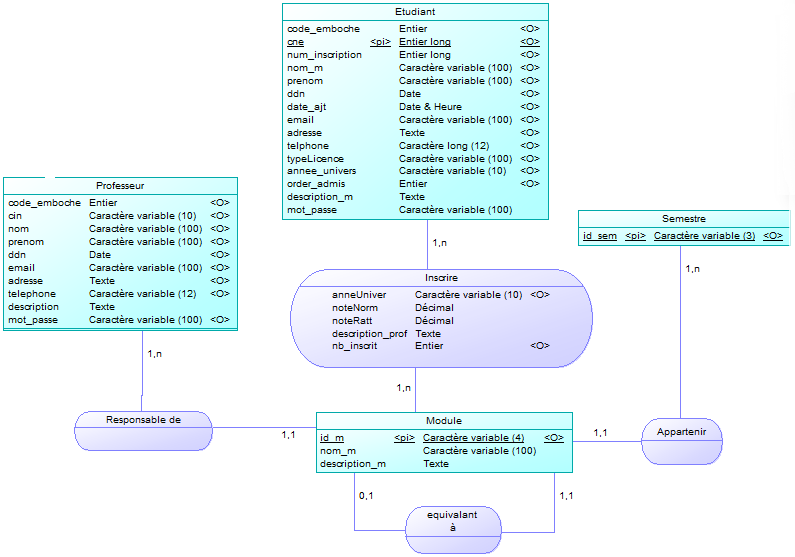
\includegraphics[width=13cm, height=7cm]{images/clientCaptures/mcd.png}
\end{alertblock}
\end{column}
\end{columns}
\end{frame}

\begin{frame}
\frametitle{Coté fournisseur (Python)}
\framesubtitle{modèles Soap (wsmodels.py)}
%\transblindsvertical[duration=1]
\transsplitverticalout[duration=1.5]
Dans \textcolor{deepgreen}{Soaplib}, les types sont les composants responsables de la conversion des paramètres individuels depuis et vers \textcolor{deepblue}{XML}, ainsi que la fourniture des informations nécessaires pour construire le \textcolor{deepblue}{WSDL}. \textcolor{deepgreen}{Soaplib} a beaucoup de types intégrés qui vous donnent la plupart des types de données communs généralement nécessaires.
\end{frame}


\begin{frame}
\frametitle{Coté fournisseur (Python)}
\framesubtitle{Service Etudiant (views.py)}
%\transblindsvertical[duration=1]
\transsplitverticalout[duration=1.5]
Ce fichier contient généralement les différents services. Dans notre cas il ne contient qu'un seul service \textcolor{backgroundcolor}{\textbf{EtudiantService}} et ses méthodes que le client va les appeler.
\end{frame}

\subsection{Coté Consommateur}
\begin{frame}
\frametitle{Coté Consommateur (Java)}
\framesubtitle{Créer projet (Netbeans)}
%\transblindsvertical[duration=1]
\transboxin[duration=1]
\begin{columns}
\begin{column}{16cm}
 \begin{alertblock}{Créer nouveau projet}
 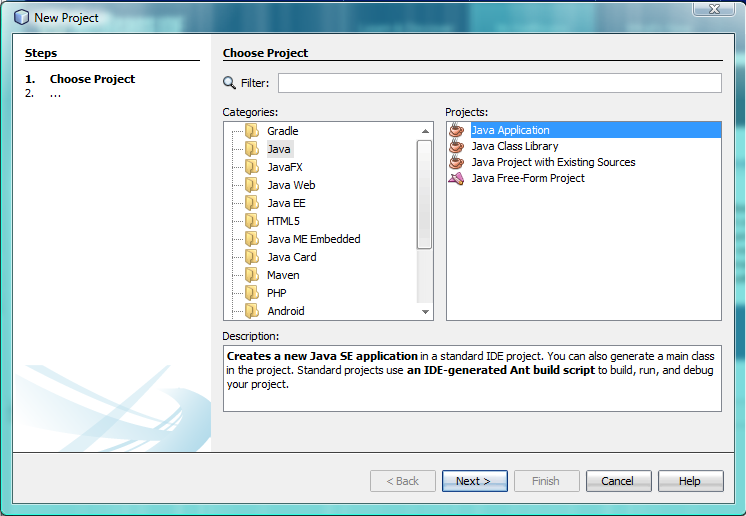
\includegraphics[width=16cm,height=7.2cm]{images/clientCaptures/etape1_new_project.png}
  \end{alertblock}
\end{column}
\end{columns}
\end{frame}

\begin{frame}
\frametitle{Coté Consommateur (Java)}
\framesubtitle{Créer projet (Netbeans)}
%\transblindsvertical[duration=1]
\transsplithorizontalin[duration=1]
\begin{columns}
\begin{column}{16cm}
 \begin{alertblock}{Créer nouveau projet}
 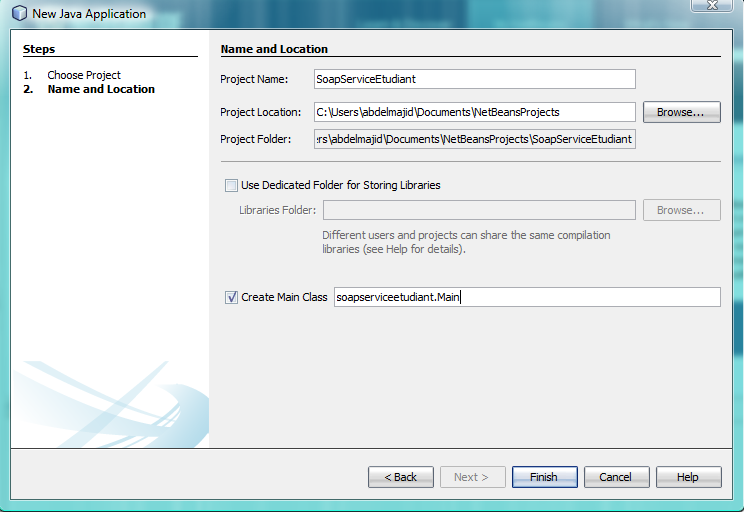
\includegraphics[width=16cm,height=7.2cm]{images/clientCaptures/etape2_new_project.png}
  \end{alertblock}
\end{column}
\end{columns}
\end{frame}


\begin{frame}
\frametitle{Coté Consommateur (Java)}
\framesubtitle{Importer au sein du projet un web service (Netbeans)}
%\transblindsvertical[duration=1]
\transsplithorizontalin[duration=1]
\begin{columns}
\begin{column}{16cm}
 \begin{alertblock}{Créer un Web Service Client}
 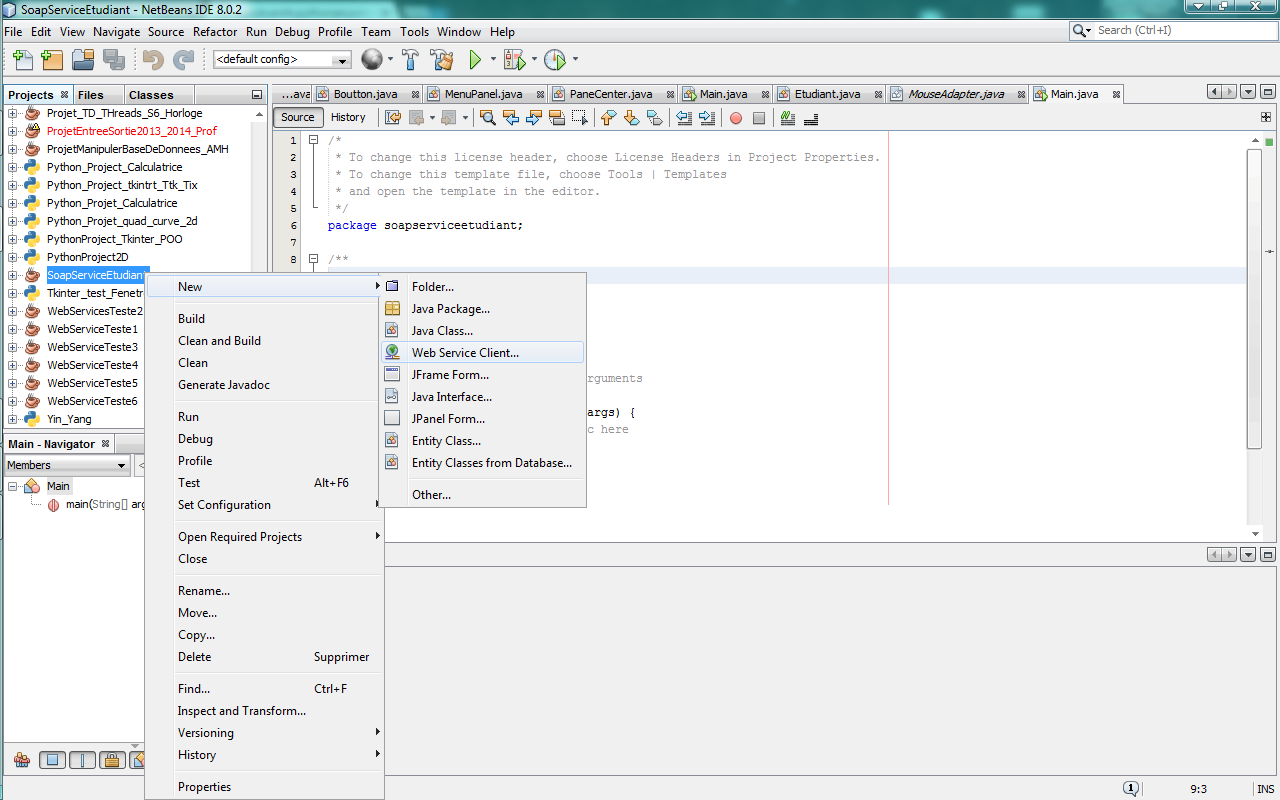
\includegraphics[width=16cm,height=7.2cm]{images/clientCaptures/etape3_client_web_service.png}
  \end{alertblock}
\end{column}
\end{columns}
\end{frame}

\begin{frame}
\frametitle{Coté Consommateur (Java)}
\framesubtitle{Préciser l'url du ficher WSDL (Netbeans)}
%\transblindsvertical[duration=1]
\transsplithorizontalin[duration=1]
\begin{columns}
\begin{column}{16cm}
 \begin{alertblock}{Url du fichier WSDL}
 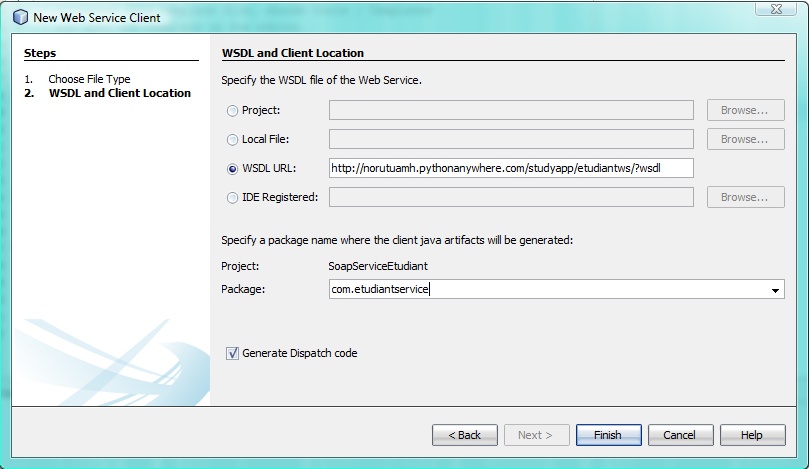
\includegraphics[width=16cm,height=7.2cm]{images/clientCaptures/etape5_client_web_service_wsdl.png}
  \end{alertblock}
\end{column}
\end{columns}
\end{frame}

\begin{frame}
\frametitle{Coté Consommateur (Java)}
\framesubtitle{Composantes importées (Netbeans)}
%\transblindsvertical[duration=1]
\transsplithorizontalin[duration=1]
\begin{columns}
\begin{column}{10cm}
 \begin{alertblock}{}
 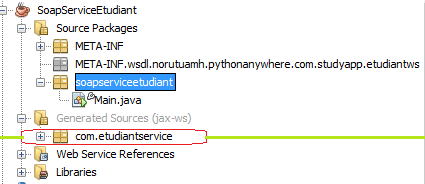
\includegraphics[width=10cm,height=5cm]{images/clientCaptures/etape6_projet_genere.png}
  \end{alertblock}
\end{column}
\end{columns}
\end{frame}

\begin{frame}
\frametitle{Coté Consommateur (Java)}
\framesubtitle{Package contenant les différents types et fonctions du WS (Netbeans)}
%\transblindsvertical[duration=1]
\transsplithorizontalin[duration=1]
\begin{columns}
\begin{column}{8cm}
 \begin{alertblock}{}
 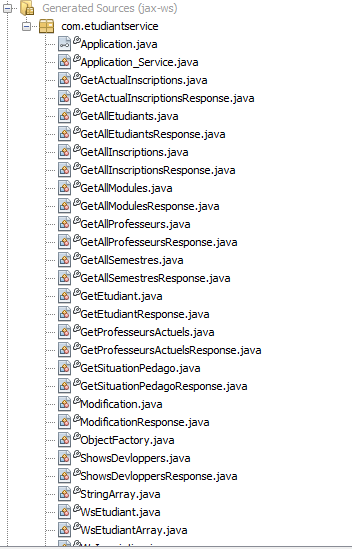
\includegraphics[width=8cm,height=8cm]{images/clientCaptures/etape7_package_fonctions_responses_types.png}
  \end{alertblock}
\end{column}
\end{columns}
\end{frame}

\begin{frame}
\frametitle{Coté Consommateur (Java)}
\framesubtitle{Contenu d'application de web service (Netbeans)}
%\transblindsvertical[duration=1]
\transsplithorizontalin[duration=1]
\begin{columns}
\begin{column}{14cm}
 \begin{alertblock}{Les opérations ou bien les fonctions du WS}
 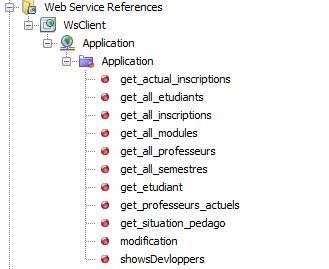
\includegraphics[width=14cm,height=7cm]{images/clientCaptures/etape8_servives_utilisess.png}
  \end{alertblock}
\end{column}
\end{columns}
\end{frame}

\begin{frame}
\frametitle{Coté Consommateur (Java)}
\framesubtitle{Compléter le projet Java (Netbeans)}
%\transblindsvertical[duration=1]
\transsplithorizontalin[duration=1]
\begin{columns}
\begin{column}{16cm}
 \begin{alertblock}{Importer une fonction dans notre projet Java.}
 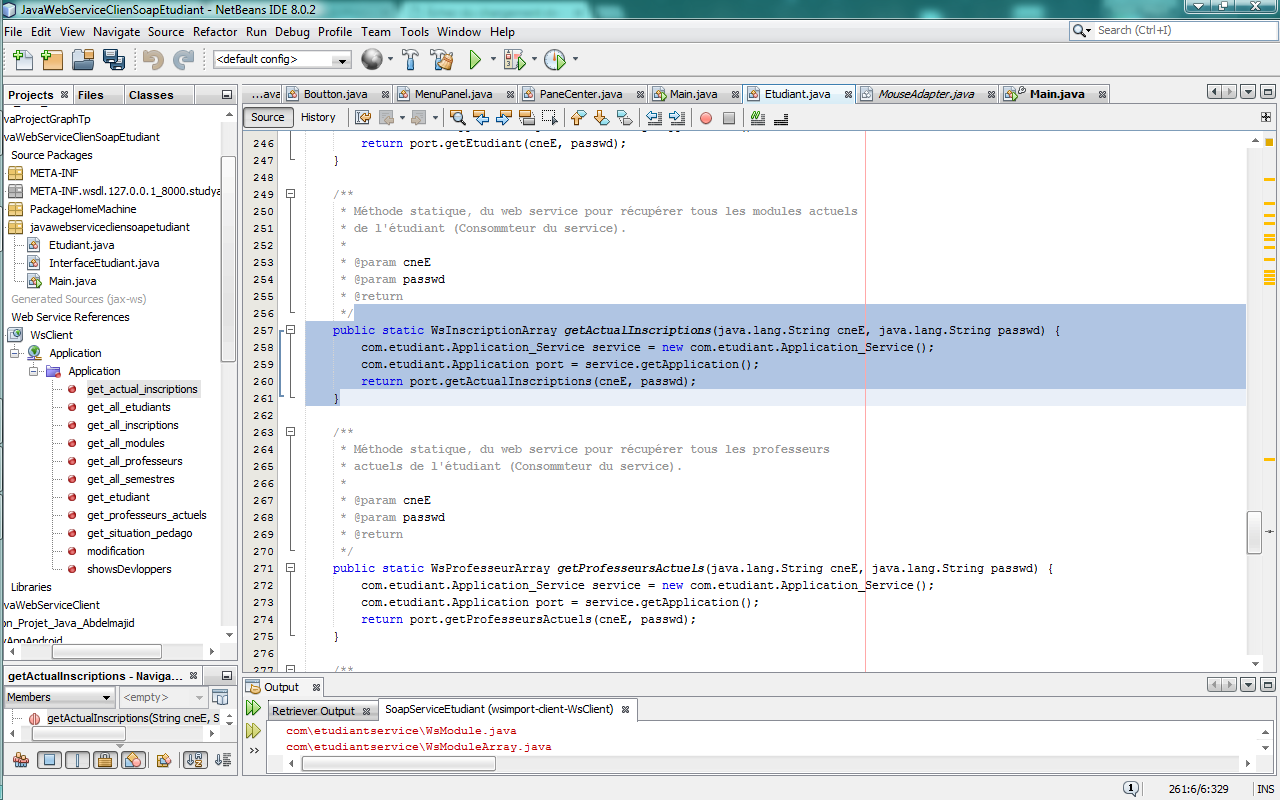
\includegraphics[width=16cm,height=7.2cm]{images/clientCaptures/etape9_importer_procedure.png}
  \end{alertblock}
\end{column}
\end{columns}
\end{frame}

